\begin{frame}
\frametitle{Page Fault}
\begin{itemize}
  \item Ошибки трансляции адресов:
  \begin{itemize}
    \item при трансляции адресов бит P может быть сброшен в одной из записей;
    \item может произойти нарушение привелегий - непривилегированный код
    пытается читать/писать память только для привилегированного кода;
    \item нарушение прав доступа, запись/исполнение в/из памяти доступной только
    на чтение.
  \end{itemize}
  \item При подобных ошибках полезно знать:
  \begin{itemize}
    \item адрес, к которому происходило обращение;
    \item какое обращение к памяти происходило (чтение/запись/исполнение) или
    какого рода ошибка произошла.
  \end{itemize}
\end{itemize}
\end{frame}

\begin{frame}
\frametitle{Page Fault в x86}
\framesubtitle{Код ошибки при Page Fault}
\begin{center}
  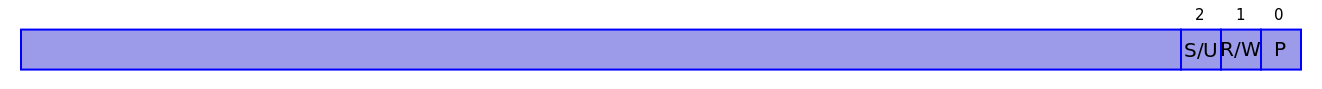
\includegraphics[width=0.9\linewidth]{pferr.png}
\end{center}
\begin{itemize}
  \item P - 0, если Page Fault произошел из-за сброшенного бита P в одной из
  записей;
  \item R/W - 0, если Page Fault произошел при чтении, в проивном случае Page
  Fault произошел при запси;
  \item S/U - 0, если Page Fault произошел в привилегированном коде, в противном
  случае Page Fault произошел в непривилегированном коде.
\end{itemize}
\end{frame}

\begin{frame}
\frametitle{Page Fault в x86}
\framesubtitle{Адрес доступа и адрес возврата}
\begin{itemize}
  \item Адрес, обращение к которому вызвало Page Fault, сохраняется в
  специальный регистр \emph{cr2}.
  \item Адрес возврата, который сохраняется на стек перед вызовом обработчика
  исключения, содержит адрес инструкции, которая привела к Page Fault
  \begin{itemize}
    \item т. е. по возращению из обработчика исключения инструкция будет
    выполнена заново;
    \item т. е. обработчик исключения может поправить отображение после чего
    инструкция будет выполнена заново.
  \end{itemize}
\end{itemize}
\end{frame}

\begin{frame}
\frametitle{Page Fault в x86}
\framesubtitle{Пример: оптимизация memcpy больших регионов 1/3}
\begin{center}
  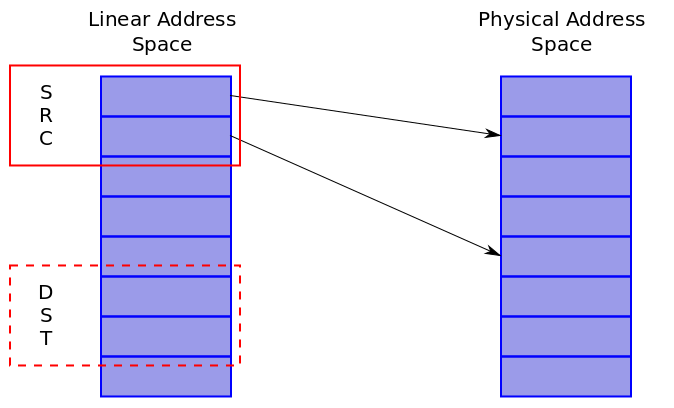
\includegraphics[width=0.6\linewidth]{memcpy0.png}
\end{center}
\begin{itemize}
  \item Хотим скопировать SRC в DST (для простоты регионы выровнены на 4 KB)
  \begin{itemize}
    \item SRC каким-то образом отображено на физическую память;
    \item отображение DST нас не особо интересует.
  \end{itemize}
\end{itemize}
\end{frame}

\begin{frame}
\frametitle{Page Fault в x86}
\framesubtitle{Пример: оптимизация memcpy больших регионов 2/3}
\begin{center}
  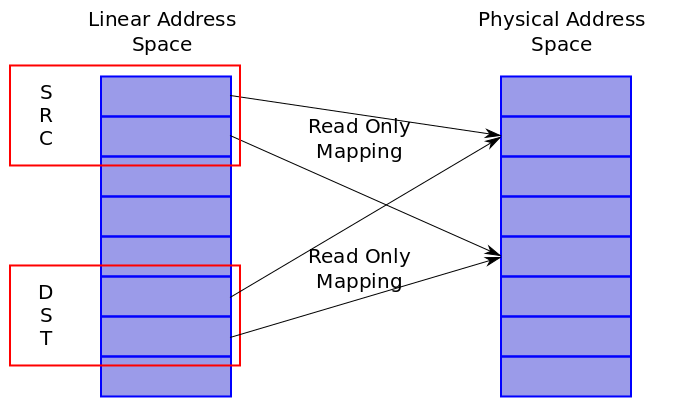
\includegraphics[width=0.6\linewidth]{memcpy1.png}
\end{center}
\begin{itemize}
  \item Вмеcто копирования памяти отображаем DST на те же страницы, что и SRC
  \begin{itemize}
    \item оба оторбажения должны быть Read Only, чтобы модификация приводила к
    Page Fault.
  \end{itemize}
\end{itemize}
\end{frame}

\begin{frame}
\frametitle{Page Fault в x86}
\framesubtitle{Пример: оптимизация memcpy больших регионов 3/3}
\begin{center}
  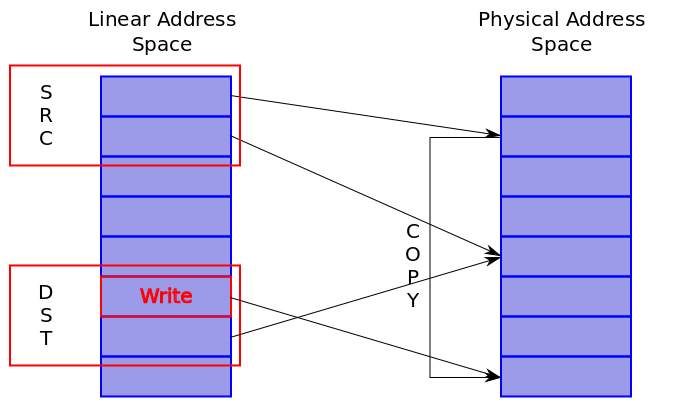
\includegraphics[width=0.6\linewidth]{memcpy2.png}
\end{center}
\begin{itemize}
  \item Попытка записи в SRC или DST приводит к Page Fault:
  \begin{itemize}
    \item в обработчике Page Fault мы можем на самом деле скопировать страницу
    памяти;
    \item таким образом мы реально копируем только те страницы, которые будут
    изменяться и только тогда, когда они будут изменяться.
  \end{itemize}
\end{itemize}
\end{frame}

